%\documentclass[]{spie}  %>>> use for US letter paper
\documentclass[a4paper,nocompress]{spie}  %>>> use this instead for A4 paper
%\documentclass[nocompress]{spie}  %>>> to avoid compression of citations

\renewcommand{\baselinestretch}{1.0} % Change to 1.65 for double spacing
 
\usepackage{amsmath,amsfonts,amssymb}
\usepackage{graphicx}
\usepackage[colorlinks=true, allcolors=blue]{hyperref}
\usepackage[dvipsnames]{xcolor}
\usepackage{tabularx}
\setlength{\extrarowheight}{2pt}
\usepackage{chemformula}

\title{Quantifying the Impact \\ of Performance Improvements and Cost Reductions \\ from 20 years of Light-Emitting Diode Manufacturing}

\author[a,b]{Michael Weinold}
\author[b]{Sergey Kolesnikov}
\author[c]{Laura Diaz Anadon}
\affil[a]{ETH Zurich, Chair of Entrepreneurial Risks, Scheuchzerstrasse 7, 8092 Zurich, Switzerland}
\affil[b]{University of Cambridge, Centre for Environment, Energy and Natural Resource Governance, The David Attenborough Building, CB2 3QZ Cambridge, UK}

\authorinfo{Further author information: (Send correspondence to Michael Weinold)\\Michael Weinold: E-mail: michael.weinold@alumni.ethz.ch}

% Option to view page numbers
\pagestyle{empty} % change to \pagestyle{plain} for page numbers   
\setcounter{page}{301} % Set start page numbering at e.g. 301
 
\begin{document} 
\maketitle

\begin{abstract}
We collected historical data on device performance, technological breakthroughs and manufacturing innovation for phosphor-converted white light-emitting diodes for the past 20 years. We used this information to identify and quantify the principal sources of performance improvements in LED manufacturing. We found that in order to quantify the impact of single technological changes, it is necessary to analyse performance improvements the device sub-efficiency level. We further developed a bottom-up manufacturing cost model with process step resolution that captures improvements in throughput, yield and related costs of all relevant manufacturing steps, as well as economies of scale to analyse cost reductions and their sources. It covers progress from early manufacturing in 2003 to today. We found that larger wafer sizes have been largely responsible for cost reductions. We found that XXX well known XXX.

\end{abstract}

% Include a list of keywords after the abstract 
\keywords{light-emitting diodes, innovation, efficiency, cost}

\section{INTRODUCTION}
\label{sec:intro}  % \label{} allows reference to this section

\clearpage
\section{METRICS}

Data is readily available for metrics describing overall device performance. Luminous efficacy of devices as well as total flux per device can be extracted from datasheets, together with electrical device parameters. However, 

For instance, a highly cited and frequently updated metric is the total flux per package \cite{Liu2009,haitz2011solid,cho2017white,Fontoynont2018}. In combination with the cost per total flux, this visualization is sometimes referred to as \textit{"Haitz's Law"}, in reference to an early report on LED development by Haitz et al. \cite{haitz1999case}. However, while these metrics are often used to showcase technological progress in light-emitting diode design and manufacturing, they have limited significance XXX. Firstly, it is not desirable in all applications to increase the total flux per device beyond a certain point. Reasons for limiting the total flux per device may include lighting design considerations to reduce glare \cite{khan2015led}, device efficiency considerations to avoid electrical droop at high operating currents associated with high brightness \cite{Piprek2010} and economical considerations where multiple LED die in a single package can achieve the same brightness as a single high-brightness LED die. Secondly, even if one were to disregard these limitations, the total flux per device would only be a proxy for technological improvements in light-emitting diodes, if it was referring to single chips, instead of multi-chip paackages. 
Figure \ref{fig:haitz} shows an updated and expanded overview of best performing devices, both at the chip and package level, inspired by \textit{"Haitz's Law"}. It is evident that the historical improvement in total flux per package for single chips is not as pronounced as for multi-chip packages. While \textit{"Haitz's Law"} remains a popular visualization related to the progress in light-emitting diode design and manufacturing, care must be taken to consider its limitations.

\begin{figure} [ht]
    \begin{center}
        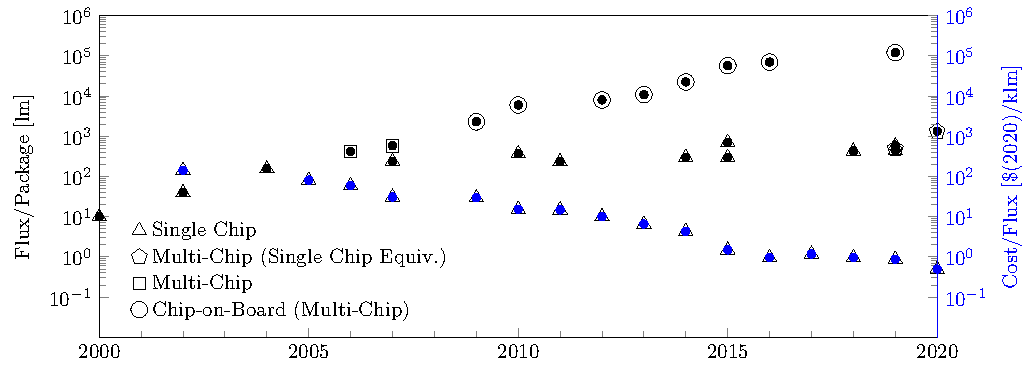
\includegraphics[width=\textwidth]{haitz_law_white.pdf}
    \end{center}
    \caption{Historical increase in flux for highest performing white light-emitting diode \underline{chips and (multi-chip) packages}, inspired by \textit{"Haitz's Law"}. Note that the increase in flux per single chip is not increasing as starkly as the flux for multi-chip packages. Shown are datapoints for best commercial performers from press releases, datasheets and and industry periodicals. Note the logarithmic ordinates and the black colored datapoints corresponding to the left ordinate, grey colored datapoints corresponding to the right ordinate. Sources: Data from Weinold et al. \cite{weinold2020technology}}
    \label{fig:haitz}
\end{figure}

Overall efficiency is cumulative from many sub-efficiencies caused by different physical effects \cite{schubert2018light}
In order to quantify the effect of single technological improvements on overall device performance, one must instead consider the metrics directly describing the various physical loss channels. Table \ref{tab:eff} lists the relevant sub-efficiencies considered along with mathematical definitions. The cumulative total lamp efficiency, defined as the product of all sub-efficiencies thus $\eta_L = \prod_{i=(V_f,\dots,S)} \eta_i$ XXX

The overall efficiency of a light-emitting diode is the product of the sub-efficiencies associated with an ensemble of different loss channels. Sub-efficiencies directly capture the effect of technology breakthroughs in device design and manufacturing process improvements. They thus provide the best metric to quantify technology breakthroughs.



        It describes the electrical and optical losses within the device, as well as the conversion losses in the phosphor layer. It further considers the mismatch between the device spectrum and an optimal spectrum, accounting for the wavelength dependent sensitivity of the human eye.

    \begin{table}[h!]
        \caption{List of the device sub-efficiencies used in our methodology. We follow the definitions used by previous authors, such as Tsao et al. \cite{tsao2010solid} and Pattison et al. \cite{pattison2017solid}. The historical development of the sub-efficiencies is displayed in figure \ref{fig:efficiency}. \\ *Also called "lamp efficiency" or "cumulative efficiency" by authors, such as Tsao et al. \cite{tsao2010solid}}
        \bigskip
        \centering
    	\begin{tabularx}{\textwidth}{|l|l|l|X|}
    		\hline
    			\textit{Symbol} & \textit{Sub-Efficiency} & \textit{Loss-Channel} & \textit{Definition} \\
    		\hline
    		    $\eta_{V_f}$ & Forward Voltage Efficiency* & Ohmic Resistance & $\eta_{V_f} = E_{h\nu} / V_f $ \\
    		\hline
    		    $\eta_{LE}$ & Light-Extraction Efficiency & Re-absorption and Reflection & $\eta_{LE}= P_{out} / P_{in} $ \\
    		\hline
    		    $\eta_{IQ}$ & Internal Quantum Efficiency & Non-radiative Recombinations & $\eta_{EQ} = \eta_{IQ} \times \eta_{LE}$ \\
    		\hline
    		    $\eta_{Droop}$ & (Electrical) Droop & Non-radiative Recombinations & $\eta_{Droop} = 1 - \eta_{IQE} / \eta_{IQE}(A \rightarrow 0) $ \\
    		\hline
    		    $\eta_C$ & Conversion Efficiency & Stokes Loss, Absorption, etc. & $\eta_{C} = E_{\textcolor{blue}{B}} / \sum_{i=\textcolor{red}{R},\textcolor{orange}{O},\textcolor{yellow}{Y},\textcolor{teal}{G}} E_i$ \\
    		\hline
    		    $\eta_{S}$ & Spectral Efficiency & Eye Sensitivity & $\eta_{S} = K / K_{max}(CRI,CCT)$ \\
    		\hline
    		    $\eta_L$ & Lamp Efficiency & N/A (Cumulative) & $\eta_L = \prod_{i=(V_f,\dots,S)} \eta_i$ \\
            \hline
                \multicolumn{4}{|l|}{$\!\begin{aligned}
                    E_{h\nu} &\dots \text{photon energy} \\
                    V_f &\dots \text{forward voltage} \\
                    A &\dots \text{electrical current} \\
                    E_{B,\dots,G} &\dots \text{optical energy of monochromatic light (blue, red, orange, yellow, green)} \\
                    K &\dots \text{luminous efficacy of radiation} \\
                    CRI &\dots \text{color rendering index}, \ CCT \dots \text{color temperature} \\
                \end{aligned}$} \\
            \hline
    	\end{tabularx}
    	\label{tab:eff}
    \end{table}

consumer experience important
metrics relevant to consumer experience
some are contested
consumer experience metrics have been trated in my thesis \cite{weinold2020technology}.
flicker is out of scope and has been treated in a separate publication
Flicker \cite{weinold2020long}

\begin{figure} [ht]
    \begin{center}
        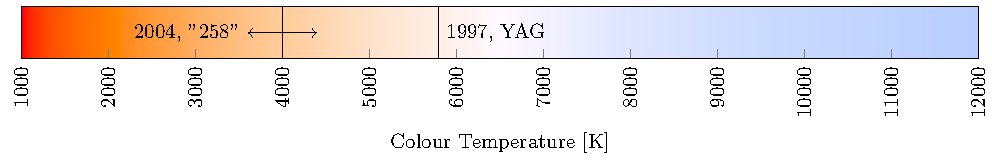
\includegraphics[width=\textwidth]{SPIE/article/cct_spectrum.pdf}
    \end{center}
    \caption{Color temperature for temperature values between 1,000K and 12,000K. Vertical lines indicate the color temperature of blue light emitting diodes used in combinations with phosphors. Two data points are shown: The 1997 \textit{Nichia} \ch{YAG:Ce^{3+}} (YAG) phosphor at 5800K and the 2004 \textit{Lumileds} \ch{Sr_2Si_5N_8:Eu^{2+}} ("258") phosphor at below 4000K. Color data generated using the \textit{luxpy} package for \textit{Python}. CCT for phosphors computed using the \textit{color science} package for \textit{Python}, from spectral data in publications  \cite{bando1998development,MuellerMach2005}.}
    \label{fig:cct}
\end{figure}

\clearpage
\section{METHODS}
\label{sec:methods}

To quantify changes in the manufacturing cost of devices, a bottom-up manufacturing cost model with process step resolution was constructed to cover the entire manufacturing process of GaN-on-sapphire based phosphor converted low-to-mid power light-emitting diode packages of different chip architectures. We considered classical p-side-up lateral current spreading devices, as well as a packaged flip-chip vertical current spreading architecture and a chip-scale package flip chip architecture. The model was constructed for the years 2003, 2012 and 2020. It was populated with equipment data from European and North American firms, selected for a virtual North American manufacturing location. Process specific step parameters were derived from scientific literature, company publications, archived product catalogs and patent literature. Details of the manufacturing process, as well as changes in the same were gathered from detailed patent analysis, augmented by interviews with experts from industry and academia. For 2012, data for the model was adapted from the \textit{LEDCOM} cost model prepared for the US Department of Energy by Stephen Bland. The model includes both the wafer treatment process as well as the packaging process. It is important to note that the aim of the model is not to faithfully represent real world manufacturing conditions in Asia based plants, but rather to show the effect of single technological changes in the manufacturing process on total cost. This means that while the model does consider overhead costs and depreciation, it does so only to XXXX 

    To dis-aggregate the contribution of changes in single variables on total performance in both the device sub-efficiencies and the manufacturing cost, we used an approach introduced by Kavlak et al. \cite{kavlak2018evaluating}. It is based on the logarithmic derivative of the total differential of the cost function. We can write the cost function $C$ of the manufacturing process as a function of a vector of cost model variables $\vec{r}=(r_1,r_2,\dots)$, where $g_{iw}(r_w)$ gives the dependence of $i$th cost component on the $w$th variable. The contribution of changes in the cost model $\Delta C_z$ to total manufacturing cost $C$ can now be approximated. For the detailed derivation, we refer to the supplementary material of the original publication.

	\begin{align}
        C(\vec{r}) &= C(r_1,r_2, \dots) = \sum_i C_i = \sum_i C_i^0 \prod_w g_{iw}(r_w) \\
        \Delta C_x &= \int_{t=t_0}^{t_1} C(t) \frac{ \partial \ln C }{ \partial x } \frac{ \text{d} x }{ \text{d} t} \text{d} t \\
        \Delta C_z (t_1,t_2) &\approx \sum_i \tilde{C_i} \ln \frac{g_{iz}(t_2)}{g_{iz}(t_1)}
    \end{align}
    
To gain a detailed understanding of the sources and magnitude of efficiency improvements in devices, we gathered data on overall device performance and identified the associated device architecture and types of down conversion phosphors used. We systematically identified the improvements related to each device sub-efficiency, gathered associated efficiency data from literature or computed the respective values from raw data.
For instance, in the case of spectral efficiency and the performance related to consumer experience metrics, we identified the prevalent red and yellow phosphors used during the period of interest. We then computed luminous efficacy of radiation as well as the color rendering index and color temperature from the spectral data. The development history of each phosphor was researched to determine if it had been developed specifically for use in light emitting devices, or if it was instead the result of a knowledge spillover.


\begin{figure} [ht]
    \begin{center}
        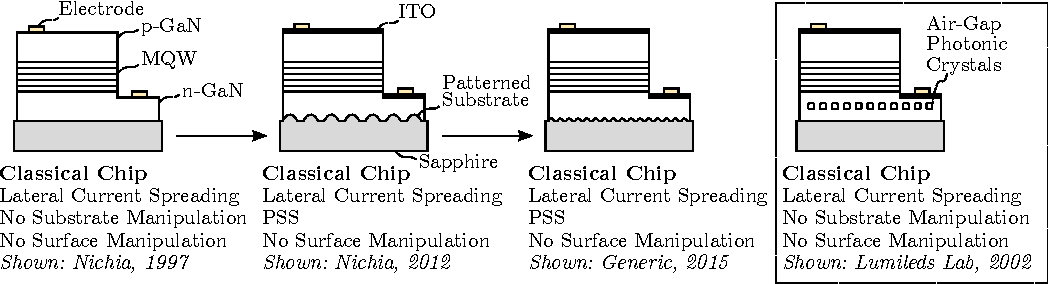
\includegraphics[width=\textwidth]{SPIE/article/chip_architectures.pdf}
    \end{center}
    \caption{Cutaway side views of the evolution of chip architectures for classical chip designs (lateral current spreading). Note that dimensions are not to scale and smaller features are greatly exaggerated for visibility. Years correspond to earliest identified patent priority date. Dashed boxes indicate chip designs not brought to large scale production. Adapted from patents \cite{nagahama2013nitride,tanaka2010semiconductor,wierer2006photonic}}
    \label{fig:chip_arch}
\end{figure}

\begin{figure} [ht]
    \begin{center}
        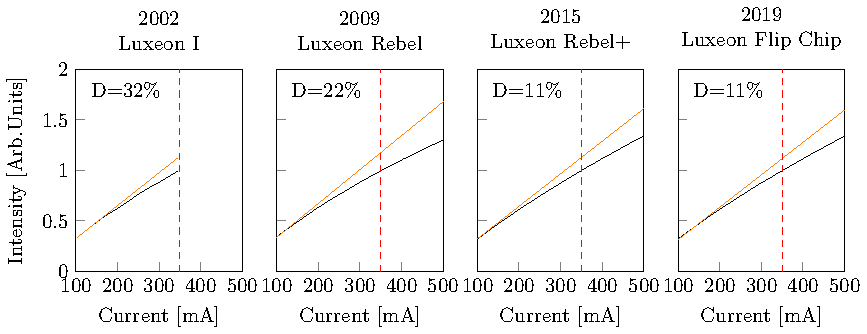
\includegraphics[width=0.85\textwidth]{SPIE/article/droop_lumileds.pdf}
    \end{center}
    \caption{Luminous intensity of four different \textit{Lumileds} high-power light-emitting diodes normalized to the value at a test current of $A_{test}=350$mA. The black curves describe the real measured intensity, the orange curves describe the estimated ideal intensity. Droop is the difference between these curves at the test current. Current-Intensity data extracted from device datasheets \cite{datasheet_lumileds_lux1,datasheet_lumileds_rebel,datasheet_lumileds_rebplus,lumi2019data}}
    \label{fig:chip_arch}
\end{figure}

\section{PERFORMANCE IMPROVEMENTS}

\begin{figure} [ht]
    \begin{center}
        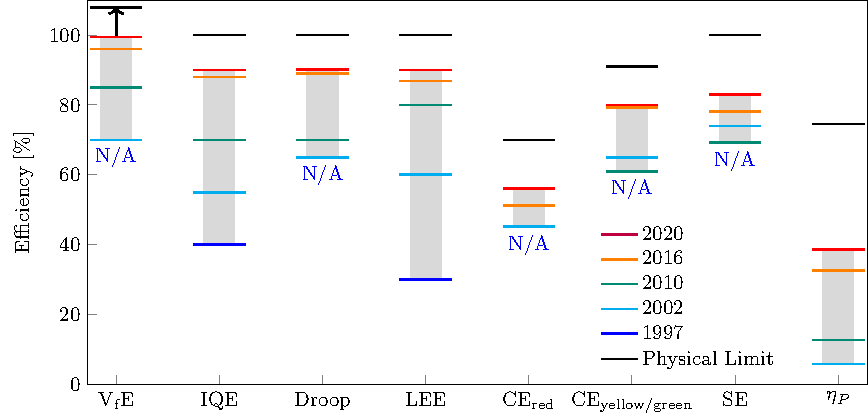
\includegraphics[width=0.85\textwidth]{SPIE/article/breakthroughs_efficiency.pdf}
    \end{center}
    \caption{Impact of technology breakthroughs and manufacturing process improvements on historical improvements in sub-efficiencies of phosphor-converted warm white light-emitting diodes with test currents of at least $I_\text{test}=350$mA. The overall lamp efficiency $\eta_L$ is displayed as the rightmost column. This figure takes as inputs the state-of-the-art sub-efficiencies discussed in section \ref{sec:methods}. Horizontal colored bars give state-of-the-art sub-efficiencies for five years: \textcolor{blue}{1997}, \textcolor{teal}{2002}, \textcolor{orange}{2010}, \textcolor{magenta}{2016} and \textcolor{red}{2020}. Colored annotation "N/A" indicates the sub-efficiency of the corresponding year cannot be computed for the following reasons: V$_\text{f}$E, Droop: depend on current, which was below 350mA at the time; CE, SE: warm white spectrum LEDs not available at the time. Physical limits are indicated by black horizontal bars. The possible range for the physical limit of V$_\text{f}$E exceeds 100\% and depends on electrical device parameters, which are discussed in \cite{david2016electrical}. The range is given by an upward pointing black arrow. Color of vertical bars indicates improvement through either technology spillovers or other improvements (technology breakthroughs or process learning). Spillovers are annotated and listed in an inset table. Efficiency acronyms: forward voltage efficiency (V$_\text{f}$E), internal quantum efficiency (IQE), light extraction efficiency (LEE), conversion efficiency (CE), spectral efficiency (SE), power conversion efficiency ($\eta_{PC}$). Spillover acronyms: patterned sapphire substrate (PSS), indium tin oxide (ITO). Data for historical improvements of sub efficiencies from Weinold et al. \cite{weinold2020technology}}
    \label{fig:efficiency}
\end{figure}

\subsection{Physical Efficiency}

give two waterfall diagrams (2003,2020) and give one example
example: maybe droop with associated figure. is good example of process improvements

\subsection{Consumer Experience}

List phosphors, give a short overview but do not include figures
show cct spectrum with lines of YAG and 258+ phosphors

\section{MANUFACTURING COST}

show two waterfall diagrams (2003 only). mention work in progress



\clearpage
\acknowledgments % equivalent to \section*{ACKNOWLEDGMENTS}       
 
The main author gratefully acknowledges funding by the \textit{Swiss Study Foundation} of Zurich, Switzerland. The authors further gratefully acknowledge project funding by the \textit{Alfred P. Sloan Foundation} of New York, USA.

% References
\bibliography{report} % bibliography data in report.bib
\bibliographystyle{spiebib} % makes bibtex use spiebib.bst

\end{document} 
